\chapter{牵张反射与神经信息}\label{ch:g12:stretch-reflex}

医生用一把小橡皮锤敲击你膝盖骨下方的\omterm{def:g10:muscles-and-joints:muscle}{肌腱}，
你还未感觉到任何东西，脚就已向前踢出。
从敲击到踢腿仅隔三十毫秒：对大脑而言太短，
甚至连做出决定也来不及。信号由肌肉
传至脊髓再返回——这是一个由两个\omterm{def:g12:stretch-reflex:neuron}{神经元}
及其间的一处连接组成的回路；同一回路也在你每一刻站立时，
默默维持身体直立。本章借此引入\omterm{def:g12:stretch-reflex:neuron}{神经元}、
它所携带的电信号，以及
\omterm{def:g12:stretch-reflex:neuron}{神经元}之间传递信息的化学连接处。

\section{反射弧}

\begin{definition}[反射]\label{def:g12:stretch-reflex:reflex}
称\emph{反射}\index{反射}为一种不随意的、迅速而刻板的
效应器（肌肉或腺体）对刺激所产生的反应，
由一条固定的\omterm{def:g12:stretch-reflex:neuron}{神经元}回路产生，该回路即
\emph{反射弧}\index{反射弧}，它经由脊髓
或脑干完成，无需大脑参与。
\emph{牵张反射}\index{牵张反射}是其中最简单的一种：
肌肉突然被拉长时，该肌肉随即收缩。
\end{definition}

\begin{proposition}[牵张反射的回路]\label{prop:g12:stretch-reflex:arc}
按顺序包括以下五个部分：
\begin{enumerate}
  \item \emph{感受器}：\emph{肌梭}，一种小型感觉
        器官，位于\omterm{def:g10:muscles-and-joints:muscle}{肌纤维}之间，肌肉拉长时它们亦被拉伸，
        并发出信号；
  \item \emph{感觉\omterm{def:g12:stretch-reflex:neuron}{神经元}}，其纤维自肌梭
        伸至脊髓，经背根进入；其胞体
        位于脊髓旁的一个神经节中。
  \item \emph{整合中枢}：脊髓的灰质，
        感觉纤维在此经一个\omterm{def:g12:stretch-reflex:synapse}{突触}直接与
        同一肌肉的运动\omterm{def:g12:stretch-reflex:neuron}{神经元}相连，并通过一个中间\omterm{def:g12:stretch-reflex:neuron}{神经元}，
        抑制拮抗肌的
        运动\omterm{def:g12:stretch-reflex:neuron}{神经元}；
  \item \emph{运动\omterm{def:g12:stretch-reflex:neuron}{神经元}}，其纤维经腹根
        离开脊髓，通往肌肉；
  \item \emph{效应器}：\omterm{def:g10:muscles-and-joints:muscle}{肌纤维}，它们收缩。
\end{enumerate}
敲击髌腱，拉伸大腿肌肉；其
肌梭发放信号，该肌肉的运动\omterm{def:g12:stretch-reflex:neuron}{神经元}随之兴奋，肌肉收缩，
小腿伸展，同时股后肌群接到放松的信号。
\end{proposition}
\begin{proof}[证据]
切断背根，\omterm{def:g12:stretch-reflex:reflex}{反射}即消失，而肌肉仍可
通过刺激腹根使其收缩；切断腹根，
\omterm{def:g12:stretch-reflex:reflex}{反射}同样消失，而肌肉被拉伸时感觉纤维仍
能传递信号，可见\omterm{def:g12:stretch-reflex:reflex}{反射弧}有感觉输入端与
运动输出端。脊髓与大脑离断的动物，\omterm{def:g12:stretch-reflex:reflex}{反射}依然存在，
说明大脑并非必需。用单根纤维记录，
显示肌梭的信号在拉伸后一毫秒之内出现，
而运动\omterm{def:g12:stretch-reflex:neuron}{神经元}约在感觉信号到达后
一毫秒才兴奋——这正是一个
\omterm{def:g12:stretch-reflex:synapse}{突触}的延迟。
\end{proof}

\begin{omfigure}
\begin{tikzpicture}[font=\small, >=Stealth, line cap=round]
  % spinal cord section (simplified): outer white, inner grey H
  \draw[thick, fill=omDef!6] (0,0) ellipse (2.2 and 1.5);
  \draw[thick, fill=gray!25] (-0.9,-1.0) -- (-0.9,0.3) .. controls (-0.9,0.9) .. (-0.5,1.0) -- (-0.3,0.4) -- (0.3,0.4) -- (0.5,1.0) .. controls (0.9,0.9) .. (0.9,0.3) -- (0.9,-1.0) .. controls (0.6,-1.1) .. (0.3,-0.5) -- (-0.3,-0.5) .. controls (-0.6,-1.1) .. (-0.9,-1.0) -- cycle;
  \node[font=\scriptsize] at (0,-1.25) {灰质};
  \node[anchor=south, font=\scriptsize] at (0,1.6) {脊髓（切面）};
  % sensory neuron: from spindle (right, muscle) to dorsal root (top right) into grey matter
  \draw[thick, omDef] (5.4,1.2) -- (3.2,1.2) -- (2.4,1.1);
  \draw[thick, omDef] (2.4,1.1) .. controls (1.4,0.9) .. (0.55,0.5);
  \fill[omDef] (2.7,1.2) circle (3pt); \node[font=\scriptsize, omDef, anchor=south] at (2.7,1.35) {胞体};
  \node[font=\scriptsize, omDef, anchor=south] at (4.4,1.3) {感觉神经元};
  % motor neuron: cell body in ventral grey, axon out ventral root to muscle
  \fill[omThm] (0.55,-0.7) circle (4pt);
  \draw[thick, omThm] (0.55,-0.7) .. controls (1.6,-1.2) .. (2.6,-1.3) -- (5.4,-1.3);
  \node[font=\scriptsize, omThm, anchor=north] at (4.2,-1.4) {运动神经元};
  % synapse mark
  \fill[omProp] (0.55,0.5) circle (2pt); \draw[omProp, thick] (0.55,0.45) -- (0.55,-0.6);
  \node[font=\scriptsize, omProp, anchor=west] at (1.0,-0.15) {突触};
  % interneuron to antagonist
  \fill[omMeth!70!black] (-0.5,-0.2) circle (3pt);
  \draw[thick, omMeth!70!black] (0.5,0.5) .. controls (0.0,0.4) .. (-0.5,-0.2);
  \draw[thick, omMeth!70!black, dashed] (-0.5,-0.2) .. controls (-1.3,-0.9) .. (-2.4,-1.2) -- (-3.2,-1.2);
  \node[font=\scriptsize, omMeth!70!black, anchor=north, align=center] at (-2.4,-1.35) {抑制拮抗肌的 \\ 运动神经元};
  % muscle with spindle (right)
  \draw[thick, fill=omThm!25, rounded corners=8pt] (5.4,-1.7) rectangle (7.6,1.7);
  \node[font=\scriptsize] at (6.5,-1.4) {肌肉};
  \draw[thick, fill=omDef!30] (6.5,1.2) ellipse (0.55 and 0.25);
  \node[font=\scriptsize] at (6.5,0.7) {肌梭};
  \draw[->, thick] (6.5,2.75) -- (6.5,1.85) node[pos=0, above, align=center, font=\scriptsize] {敲击肌腱：\\ 肌肉被拉伸};
  \node[font=\scriptsize, anchor=north, align=center] at (6.5,-1.85) {运动纤维止于 \\ 肌肉：收缩};
\end{tikzpicture}

{\small \omterm{def:g12:stretch-reflex:reflex}{牵张反射}弧，示于脊髓横切面中。
肌梭的感觉\omterm{def:g12:stretch-reflex:neuron}{神经元}（蓝色）经背根进入，
经一个\omterm{def:g12:stretch-reflex:synapse}{突触}（橙色）与同一肌肉的运动\omterm{def:g12:stretch-reflex:neuron}{神经元}（红色）相连，
该运动\omterm{def:g12:stretch-reflex:neuron}{神经元}经腹根离开脊髓；一个中间\omterm{def:g12:stretch-reflex:neuron}{神经元}
（绿色）抑制拮抗肌。}
\end{omfigure}

\begin{omfigure}
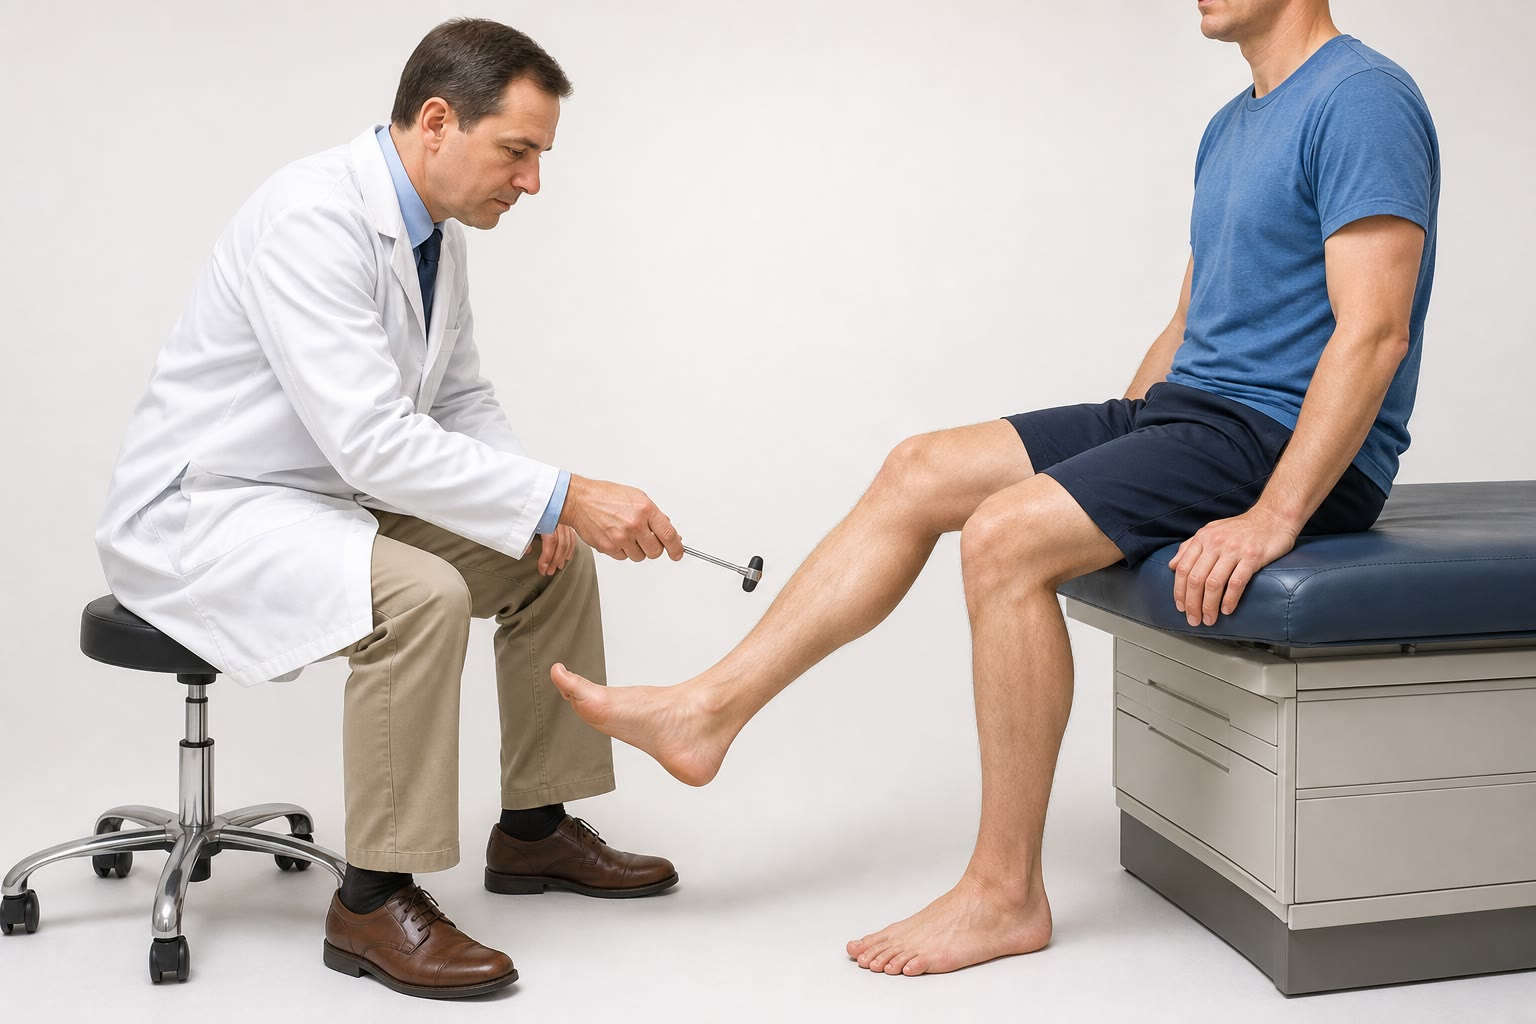
\includegraphics[width=0.56\linewidth]{images/book2/ai/g12-reflex-hammer.jpg}

{\small 膝跳\omterm{def:g12:stretch-reflex:reflex}{反射}检查：敲击髌腱，拉伸大腿肌肉，
三十毫秒后小腿踢出。该\omterm{def:g12:stretch-reflex:reflex}{反射}
在一秒之内即可检验从肌梭到肌肉的整个\omterm{def:g12:stretch-reflex:reflex}{反射弧}。}
\end{omfigure}

\begin{example}[反射的作用]\label{ex:g12:stretch-reflex:posture}
站立时，你会轻微晃动；每次晃动都会拉伸
踝部一侧的肌肉，肌梭随之发放信号，\omterm{def:g12:stretch-reflex:reflex}{反射}性收缩将你拉回，
使你在察觉之前恢复平衡。端着托盘时，突然增加的重量会拉伸
手臂肌肉，\omterm{def:g12:stretch-reflex:reflex}{反射}会在 \qty{30}{ms} 内使其僵硬，
赶在托盘倾斜之前。\omterm{def:g12:stretch-reflex:reflex}{牵张反射}是一种伺服机制：它抵抗
肌肉长度的任何变化，大脑则调节其
敏感度，以设定身体的张力——绷紧时调高，入睡时调低。
\end{example}

\section{神经元及其信息}

\begin{definition}[神经元]\label{def:g12:stretch-reflex:neuron}
\emph{神经元}\index{神经元}是一种专门用于传递信号的\omterm{def:g10:cells-common-unit:cell}{细胞}：它由
带\omterm{def:g10:cells-common-unit:organelle}{细胞核}的\omterm{def:g10:cells-common-unit:cell}{细胞}体、接收信号的分支状\emph{树突}，以及一条长长的单根纤维，
即\emph{轴突}，将神经元自身的信号传送到其末梢——
以腿部的运动神经元为例，
末梢距\omterm{def:g10:cells-common-unit:cell}{细胞}体约一米。许多轴突外包有富含\omterm{def:g10:chemistry-of-life:families}{脂质}的鞘，即\emph{髓鞘}，
由伴随\omterm{def:g10:cells-common-unit:cell}{细胞}形成，能加快传导。神经是由
数百或数千条轴突组成的束。
\end{definition}

\begin{omfigure}
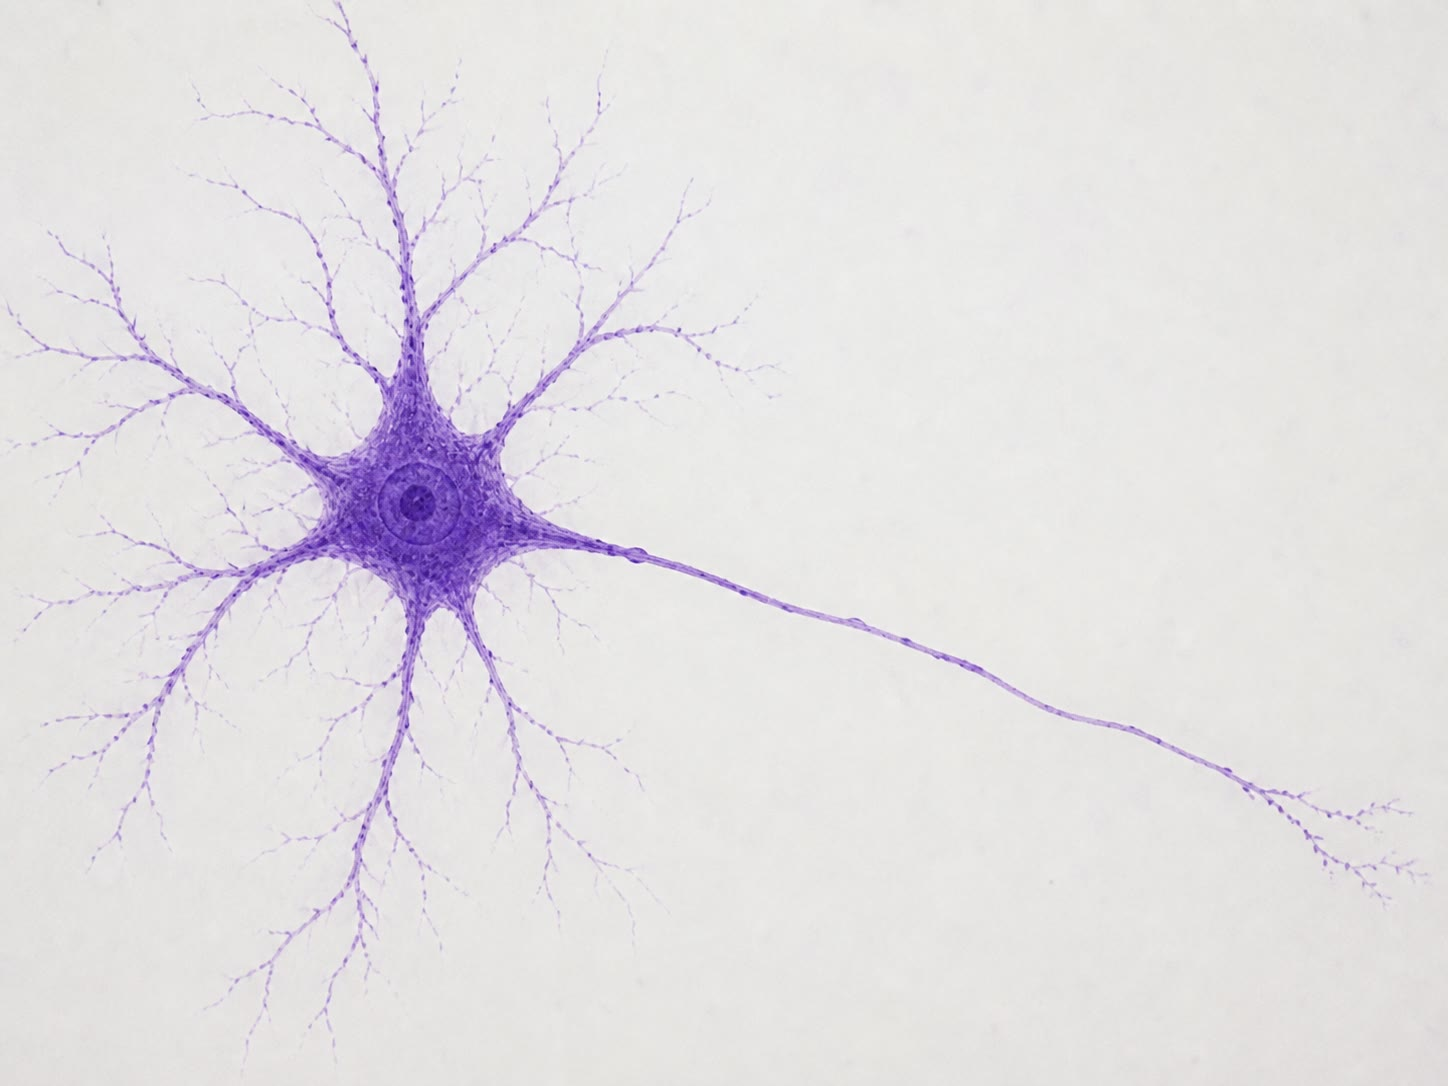
\includegraphics[width=0.5\linewidth]{images/book2/ai/g12-neuron-micrograph.jpg}

{\small 经染色的运动\omterm{def:g12:stretch-reflex:neuron}{神经元}：带\omterm{def:g10:cells-common-unit:organelle}{细胞核}的\omterm{def:g10:cells-common-unit:cell}{细胞}体，分支状的
接收信号的树突，以及将\omterm{def:g12:stretch-reflex:neuron}{神经元}自身信息传送至肌肉的单根
轴突。}
\end{omfigure}

\begin{proposition}[动作电位]\label{prop:g12:stretch-reflex:actionpotential}
\omterm{def:g12:stretch-reflex:neuron}{神经元}的膜带有电压：静息时，内侧相对外侧约为
\qty{-70}{mV}。
\emph{神经信息}\index{神经信息}是一串
\emph{动作电位}\index{动作电位}：即该电压的短暂反转，
每次上升至约 \qty{+30}{mV}，并在一毫秒内恢复，
沿轴突无衰减地传播。\omterm{prop:g12:stretch-reflex:actionpotential}{动作电位}具有\emph{全或无}性质：
低于阈值的刺激不产生任何反应，
高于阈值的任何刺激都产生同样大小的完整信号。
因此，刺激的强度并不编码在信号的大小中，
而编码在信号的\emph{频率}中：牵拉越强，
肌梭每秒发放的\omterm{prop:g12:stretch-reflex:actionpotential}{动作电位}就越多。
\end{proposition}
\begin{proof}[证据]
将微电极插入轴突，可记录静息电压，并在\omterm{def:g10:cells-common-unit:cell}{细胞}发放时
记录到形状相同的尖峰，其形状不随刺激强度或传导距离而改变。
对单根肌梭纤维在牵拉逐渐增大时进行记录，
尖峰大小恒定，而发放速率从每秒数个升至数百个。
刚低于阈值的刺激完全不产生尖峰；
对已高于阈值的刺激加倍，
只改变发放速率，不改变尖峰高度。
\end{proof}

\begin{omfigure}
\begin{tikzpicture}
\begin{axis}[
  width=0.62\linewidth, height=5.6cm,
  axis x line=bottom, axis y line=left,
  xmin=0, xmax=5, ymin=-100, ymax=50,
  xlabel={时间 (ms)}, ylabel={膜电压 (mV)},
  xlabel style={font=\small, at={(axis description cs:0.5,-0.12)}, anchor=north},
  ylabel style={font=\small},
  tick label style={font=\small}, xtick={0,1,2,3,4,5}, ytick={-70,-30,0,30},
  clip=false,
]
\addplot[thick, omThm, smooth] coordinates {(0,-70) (1,-70) (1.3,-55) (1.5,-20) (1.7,30) (1.9,10) (2.1,-40) (2.3,-75) (2.7,-80) (3.2,-72) (4,-70) (5,-70)};
\draw[dashed, gray] (axis cs:0,-55) -- (axis cs:5,-55);
\node[font=\scriptsize, gray, anchor=south west] at (axis cs:3.3,-55) {阈值};
\node[font=\scriptsize, anchor=south west] at (axis cs:0.1,-68) {静息};
\node[font=\scriptsize, anchor=west] at (axis cs:1.8,32) {峰值};
\end{axis}
\end{tikzpicture}

{\small 在轴突内记录到的\omterm{prop:g12:stretch-reflex:actionpotential}{动作电位}：自静息的
\qty{-70}{mV}起，迅速上升越过阈值至约 \qty{+30}{mV}，
随后回落至静息电位以下，并恢复——全程约两毫秒。
同一\omterm{def:g12:stretch-reflex:neuron}{神经元}的每个\omterm{prop:g12:stretch-reflex:actionpotential}{动作电位}都具有相同的形状。}
\end{omfigure}

\begin{omfigure}
\begin{tikzpicture}[font=\small, line cap=round]
  \foreach \row/\y/\lab/\n in {1/2.4/{弱牵拉}/6, 2/1.2/{中等牵拉}/12, 3/0/{强牵拉}/24} {
    \draw[thick] (0,\y) -- (9,\y);
    \node[anchor=east] at (-0.2,\y) {\lab};
  }
  \foreach \i in {1,...,6} \draw[very thick, omThm] ({\i*9/7},2.4) -- ({\i*9/7},2.4+0.6);
  \foreach \i in {1,...,12} \draw[very thick, omThm] ({\i*9/13},1.2) -- ({\i*9/13},1.2+0.6);
  \foreach \i in {1,...,24} \draw[very thick, omThm] ({\i*9/25},0) -- ({\i*9/25},0.6);
  \draw[<->] (0,-0.5) -- (9,-0.5) node[midway, below] {\qty{100}{ms}};
\end{tikzpicture}

{\small 频率编码。同一根肌梭纤维在三次牵拉下的记录：
尖峰完全相同，变化的只是发放速率——
此处分别约为每秒 60、120 和 240 次。}
\end{omfigure}

\begin{example}[速度]\label{ex:g12:stretch-reflex:speed}
\omterm{prop:g12:stretch-reflex:actionpotential}{动作电位}在细的无髓纤维中以 \qty{1}{m/s} 的速度传导，
在\omterm{def:g12:stretch-reflex:reflex}{牵张反射}所用的粗有髓纤维中可达 \qty{100}{m/s}。
从膝部到脊髓再返回，全程约 \qty{1.5}{m}：传导约需 \qty{15}{ms}，
再加上肌梭的反应、一个\omterm{def:g12:stretch-reflex:synapse}{突触}以及肌肉的激活，
又需 \qty{15}{ms}——合计即膝跳\omterm{def:g12:stretch-reflex:reflex}{反射}的 \qty{30}{ms}。
从脚趾到大脑，相距 \qty{1.8}{m}，信息约需 \qty{20}{ms}；
决定移动它，以及执行这一动作，
还需约 \qty{150}{ms}。
\end{example}

\section{突触}

\begin{definition}[突触与神经递质]\label{def:g12:stretch-reflex:synapse}
\emph{突触}\index{突触}是一个\omterm{def:g12:stretch-reflex:neuron}{神经元}轴突的末梢与下一个\omterm{def:g10:cells-common-unit:cell}{细胞}相接之处，
即另一个\omterm{def:g12:stretch-reflex:neuron}{神经元}或\omterm{def:g10:muscles-and-joints:muscle}{肌纤维}，两者之间隔着
约 \qty{20}{nm} 的间隙，即\emph{突触间隙}。信号并非以电的方式跨越间隙：到达的
\omterm{prop:g12:stretch-reflex:actionpotential}{动作电位}使末梢从小囊泡中释放一种化学信使，
即\emph{神经递质}\index{神经递质}，释放进入
突触间隙中；它与接收\omterm{def:g10:cells-common-unit:cell}{细胞}膜上的\emph{受体}结合，
使该\omterm{def:g10:cells-common-unit:cell}{细胞}的电压发生改变；随后它在毫秒之内被分解或
回收。突触把电信息转换为化学信息，再转换回电信息，
而释放的递质量——由到达的\omterm{prop:g12:stretch-reflex:actionpotential}{动作电位}频率决定——
编码了
信息的
强度。
\end{definition}

\begin{omfigure}
\begin{tikzpicture}[font=\small, >=Stealth, line cap=round]
  % presynaptic ending
  \draw[thick, fill=omDef!12] (0,0) -- (3.0,0) .. controls (4.0,0) and (4.0,2.6) .. (3.0,2.6) -- (0,2.6);
  \node[anchor=east, align=right, omDef!80!black] at (-0.1,1.3) {轴突末梢 \\ （动作电位 \\ 到达）};
  \foreach \x/\y in {2.2/0.7, 2.6/1.3, 2.3/1.9, 1.6/1.2, 3.1/1.0, 3.1/1.7} \draw[thick, fill=omThm!25] (\x,\y) circle (0.22);
  \node[font=\scriptsize, anchor=south] at (1.6,1.5) {小囊泡};
  % cleft
  \draw[thick, fill=omDef!12] (4.6,-0.4) -- (4.6,3.0) -- (8.5,3.0) -- (8.5,-0.4) -- cycle;
  \node[anchor=west, align=left, omMeth!70!black] at (5.0,2.45) {接收细胞 \\ （神经元或肌肉）};
  \foreach \y in {0.5,1.1,1.7} \draw[thick, fill=omMeth!40] (4.5,\y-0.15) rectangle (4.85,\y+0.15);
  \node[font=\scriptsize, anchor=west] at (5.0,1.1) {受体};
  % transmitter molecules in cleft
  \foreach \x/\y in {4.05/0.6, 4.25/1.2, 4.1/1.6, 4.3/0.9, 4.2/1.9} \fill[omThm] (\x,\y) circle (2pt);
  \node[font=\scriptsize, anchor=north, align=center] at (4.25,-0.55) {突触间隙：递质 \\ 释放后被分解};
  \draw[->, thick] (3.35,1.3) -- (3.95,1.3);
  \draw[->, thick] (4.95,2.1) .. controls (5.6,2.0) .. (6.3,1.5) node[right, font=\scriptsize] {电压变化};
\end{tikzpicture}

{\small 一个\omterm{def:g12:stretch-reflex:synapse}{突触}。到达末梢的\omterm{prop:g12:stretch-reflex:actionpotential}{动作电位}使小囊泡
释放\omterm{def:g12:stretch-reflex:synapse}{神经递质}进入\omterm{def:g12:stretch-reflex:synapse}{突触}间隙；它与接收\omterm{def:g10:cells-common-unit:cell}{细胞}上的受体结合，
使其电压改变；随后酶将其分解。信息
以化学物质的形式跨越间隙，且只能单向传递。}
\end{omfigure}

\begin{proposition}[兴奋、抑制与肌肉的接头]\label{prop:g12:stretch-reflex:junction}
根据递质及其受体的不同，\omterm{def:g12:stretch-reflex:synapse}{突触}可以
\emph{兴奋}接收\omterm{def:g12:stretch-reflex:neuron}{神经元}（使其趋近阈值）
或\emph{抑制}它（使其远离阈值）。\omterm{def:g12:stretch-reflex:reflex}{牵张反射}同时利用两者：
兴奋肌肉自身的运动\omterm{def:g12:stretch-reflex:neuron}{神经元}，抑制
拮抗肌的运动\omterm{def:g12:stretch-reflex:neuron}{神经元}（经由中间\omterm{def:g12:stretch-reflex:neuron}{神经元}）。在\emph{神经肌肉
接头}处，即运动\omterm{def:g12:stretch-reflex:neuron}{神经元}与\omterm{def:g10:muscles-and-joints:muscle}{肌纤维}之间的\omterm{def:g12:stretch-reflex:synapse}{突触}，
递质是\emph{乙酰胆碱}：运动\omterm{def:g12:stretch-reflex:neuron}{神经元}的每个\omterm{prop:g12:stretch-reflex:actionpotential}{动作电位}
都会释放足量递质，使\omterm{def:g10:muscles-and-joints:muscle}{肌纤维}兴奋并收缩。一个
运动\omterm{def:g12:stretch-reflex:neuron}{神经元}及其支配的\omterm{def:g10:muscles-and-joints:muscle}{肌纤维}构成一个\emph{运动单位}；
肌肉的肌力由同时兴奋的运动单位数目及其放电快慢决定。
\end{proposition}
\begin{proof}[证据]
将乙酰胆碱作用于\omterm{def:g10:muscles-and-joints:muscle}{肌纤维}，可使其收缩；
\emph{箭毒}是一种毒箭用毒，它与\omterm{def:g10:muscles-and-joints:muscle}{肌纤维}的乙酰胆碱
受体结合却不将其激活，使所有肌肉麻痹，
而神经仍在放电；肉毒毒素阻止小囊泡释放，
同样使肌肉麻痹；一种杀虫剂阻断了
分解乙酰胆碱的酶，使肌肉
不受控制地收缩。士的宁阻断了
脊髓的抑制性\omterm{def:g12:stretch-reflex:synapse}{突触}，使每一次牵拉都同时引起肌肉与拮抗肌收缩，
即痉挛。每种毒物都通过去除接头中的一个环节，
从而标明该环节。
\end{proof}

\begin{method}[分析反射或毒物]\label{met:g12:stretch-reflex:analyse}
\begin{enumerate}
  \item 追踪\omterm{def:g12:stretch-reflex:reflex}{反射弧}：受体、感觉\omterm{def:g12:stretch-reflex:neuron}{神经元}、中心、运动\omterm{def:g12:stretch-reflex:neuron}{神经元}、
        效应器；指出损伤或药物影响的是哪个环节。
  \item 对每个\omterm{def:g12:stretch-reflex:neuron}{神经元}，思考其编码的是什么——
        \omterm{prop:g12:stretch-reflex:actionpotential}{动作电位}的频率；在每个\omterm{def:g12:stretch-reflex:synapse}{突触}处，思考携带信息的是什么
——递质及其释放量。
  \item 对毒物，找出其作用的环节：递质的释放、
        受体、递质的分解，或抑制性\omterm{def:g12:stretch-reflex:synapse}{突触}；
        预测麻痹（信息无法通过）或
        痉挛（抑制无法发生）。
  \item 估算时间：距离除以传导速度，
        再加上每个\omterm{def:g12:stretch-reflex:synapse}{突触}约一毫秒。
\end{enumerate}
\end{method}

\begin{remark}[由相同脉冲构成的信息]\label{rem:g12:stretch-reflex:spikes}
神经系统中的每一种信息——肌梭的牵张、
视网膜感受的光、大脑发出的运动指令——都由相同的
全或无\omterm{prop:g12:stretch-reflex:actionpotential}{动作电位}构成，区别仅在于频率及承载它们的
神经纤维；信息的含义在于哪个\omterm{def:g12:stretch-reflex:neuron}{神经元}兴奋，而不在于
它发放的是什么。在每个\omterm{def:g12:stretch-reflex:synapse}{突触}处，信息都转变为一定剂量的
化学物质，这正是分子——递质、毒物、药物——
可在任何环节介入信息传递。
末章将沿着同样的脉冲与\omterm{def:g12:stretch-reflex:synapse}{突触}上行至大脑，以及
由大脑发出、再向下传回的指令。
\end{remark}

\section{练习}

\begin{exercise}[$\star$]\label{exo:g12:stretch-reflex:1}
按顺序列出\omterm{def:g12:stretch-reflex:reflex}{牵张反射}弧的五个环节。
\end{exercise}

\begin{exercise}[$\star$]\label{exo:g12:stretch-reflex:2}
描述一个\omterm{def:g12:stretch-reflex:neuron}{神经元}的各部分，以及其信息
传递的方向。
\end{exercise}

\begin{exercise}[$\star$]\label{exo:g12:stretch-reflex:3}
什么是\omterm{prop:g12:stretch-reflex:actionpotential}{动作电位}？“全或无”是什么意思，以及
强度是如何被编码的？
\end{exercise}

\begin{exercise}[$\star$]\label{exo:g12:stretch-reflex:4}
描述从\omterm{prop:g12:stretch-reflex:actionpotential}{动作电位}到达\omterm{def:g12:stretch-reflex:synapse}{突触}
至接收\omterm{def:g10:cells-common-unit:cell}{细胞}作出反应之间发生的各个过程。
\end{exercise}

\begin{exercise}[$\star$]\label{exo:g12:stretch-reflex:5}
哪种递质在神经肌肉接头处起作用，以及
箭毒和肉毒毒素各自对其有何作用？
\end{exercise}

\begin{exercise}[$\star\star$]\label{exo:g12:stretch-reflex:6}
根据频率编码图，数出各次牵拉在 \qty{100}{ms} 内的脉冲数，
并算出各自的速率。各行之间不变的是
什么？
\end{exercise}

\begin{exercise}[$\star\star$]\label{exo:g12:stretch-reflex:7}
膝跳\omterm{def:g12:stretch-reflex:reflex}{反射}的潜伏期为 \qty{30}{ms}，通路长 \qty{1.5}{m}。若
\omterm{def:g12:stretch-reflex:synapse}{突触}和肌肉激活共需 \qty{12}{ms}，
求神经纤维的传导速度。
\end{exercise}

\begin{exercise}[$\star\star$]\label{exo:g12:stretch-reflex:8}
解释为何切断背根会使\omterm{def:g12:stretch-reflex:reflex}{反射}消失，但不会使
肌肉的收缩能力消失，而切断腹根则使
两者都消失。
\end{exercise}

\begin{exercise}[$\star\star$]\label{exo:g12:stretch-reflex:9}
\omterm{def:g12:stretch-reflex:reflex}{反射}过程中为何必须抑制拮抗肌？\omterm{def:g12:stretch-reflex:reflex}{反射弧}的哪一
成分完成这一抑制，又是通过哪类\omterm{def:g12:stretch-reflex:synapse}{突触}？
\end{exercise}

\begin{exercise}[$\star\star$]\label{exo:g12:stretch-reflex:10}
强度为 2 个单位的刺激恰好达到\omterm{def:g12:stretch-reflex:neuron}{神经元}的阈值，产生一个
幅度为 \qty{100}{mV} 的\omterm{prop:g12:stretch-reflex:actionpotential}{动作电位}。预测强度为 1、
4 和 8 个单位的刺激所引起的信号。
\end{exercise}

\begin{exercise}[$\star\star$]\label{exo:g12:stretch-reflex:11}
解释为何\omterm{prop:g12:stretch-reflex:actionpotential}{神经信息}只能单向通过\omterm{def:g12:stretch-reflex:synapse}{突触}，
并为何在此处延迟约 1 毫秒。
\end{exercise}

\begin{exercise}[$\star\star\star$]\label{exo:g12:stretch-reflex:12}
一种杀虫剂阻断了分解乙酰胆碱的酶。预测
它在神经肌肉接头处的作用及对呼吸的影响，并解释
为何阻断乙酰胆碱受体的药物可
以严格测定的剂量用作解毒剂。
\end{exercise}

\begin{exercise}[$\star\star\star$]\label{exo:g12:stretch-reflex:13}
士的宁阻断脊髓中的抑制性\omterm{def:g12:stretch-reflex:synapse}{突触}。利用
\omterm{def:g12:stretch-reflex:reflex}{反射弧}，解释为何轻触随后会引发
全身抽搐。
\end{exercise}

\begin{exercise}[$\star\star\star$]\label{exo:g12:stretch-reflex:14}
髓鞘受损者的膝跳\omterm{def:g12:stretch-reflex:reflex}{反射}潜伏期为 \qty{60}{ms}，
而非 30。利用练习 7 的数据推算其传导速度，
并解释髓鞘为何重要。
\end{exercise}

\begin{exercise}[$\star\star\star$]\label{exo:g12:stretch-reflex:15}
“脊髓只是大脑与身体之间的一根电缆。”请改写
为一段正确的论述，利用\omterm{def:g12:stretch-reflex:reflex}{反射}、中间\omterm{def:g12:stretch-reflex:neuron}{神经元}和
脊髓与大脑断开的动物。
\end{exercise}

\section{周末问题：三十毫秒}

\begin{problem}[{周末问题——对膝跳反射计时并逐步拆解：
肌梭的编码、纤维的速度、突触的延迟、
接头的化学，以及可标明每一步的毒物}]
\label{pb:g12:stretch-reflex:1}
电极记录受试者大腿肌肉的电活动
（肌电图），同时叩击髌腱。该肌肉的
信号在叩击后 \qty{30}{ms} 开始出现；腿在 \qty{20}{ms}
之后移动。从\omterm{def:g10:muscles-and-joints:muscle}{肌腱}沿神经到脊髓的距离为
\qty{75}{cm}，返程相同。

\medskip
\noindent\textbf{第一部分——时序。}
\begin{enumerate}
  \item 计算\omterm{def:g12:stretch-reflex:reflex}{反射}神经通路的总长度。
  \item 设肌梭反应与肌肉激活各需
        \qty{4}{ms}，\omterm{def:g12:stretch-reflex:synapse}{突触}需 \qty{1}{ms}。\qty{30}{ms} 中
        有多少用于传导，
        传导速度为多少？
  \item 若受试者身高增加 \qty{20}{cm}，纤维相同，
        预测其潜伏期。
  \item 为何腿部在肌肉电信号开始后
        \qty{20}{ms} 才移动？
  \item 受试者被告知预期叩击，并“想着”
        制止踢腿；踢腿本身不变。借助往返脑部的
        信息时序（多出 \qty{1.2}{m} 的神经纤维，
        及若干\omterm{def:g12:stretch-reflex:synapse}{突触}）加以解释。
\end{enumerate}

\medskip
\noindent\textbf{第二部分——编码。}
肌梭纤维静息时每秒发放 20 个\omterm{prop:g12:stretch-reflex:actionpotential}{动作电位}，叩击
期间为 200 个。
\begin{enumerate}[resume]
  \item 肌梭在叩击后的
        \qty{10}{ms} 内发出多少个\omterm{prop:g12:stretch-reflex:actionpotential}{动作电位}？静息与叩击之间
        有何变化，又有何不变？
  \item 每个到达\omterm{def:g12:stretch-reflex:synapse}{突触}的\omterm{prop:g12:stretch-reflex:actionpotential}{动作电位}释放固定量的
        \omterm{def:g12:stretch-reflex:synapse}{神经递质}。叩击期间，每秒释放的\omterm{def:g12:stretch-reflex:synapse}{神经递质}
        量增加为原来的多少倍？
  \item 运动\omterm{def:g12:stretch-reflex:neuron}{神经元}仅当
        几毫秒内有足够的\omterm{def:g12:stretch-reflex:synapse}{神经递质}到达时才放电。解释为何
        静息频率不能使肌肉收缩，而叩击频率却能。
  \item 较轻的叩击每秒产生 100 个\omterm{prop:g12:stretch-reflex:actionpotential}{动作电位}。预测运动\omterm{def:g12:stretch-reflex:neuron}{神经元}的
        反应及踢腿的力度，并利用运动单位加以分析。
  \item 解释为何肌梭的信息不能编码于\omterm{prop:g12:stretch-reflex:actionpotential}{动作电位}的
        大小之中。
\end{enumerate}

\medskip
\noindent\textbf{第三部分——接头。}
\begin{enumerate}[resume]
  \item 说出神经肌肉接头处的\omterm{def:g12:stretch-reflex:synapse}{神经递质}，并描述
        其作用后的去向。
  \item 注射箭毒后，肌电图在叩击后无信号，
        但神经仍传导\omterm{prop:g12:stretch-reflex:actionpotential}{动作电位}。哪一
        步骤被阻断？
  \item 若改用肉毒毒素，肌电图与神经信号
        均与前相同。哪一步骤受阻？在实验室中如何
        区分二者？
  \item 麻醉剂阻断感觉纤维中的
        \omterm{prop:g12:stretch-reflex:actionpotential}{动作电位}。哪些记录消失，哪些仍然存在？
  \item 解释为何这三种情况都会使腿部松弛无力，
        但机制各不相同。
\end{enumerate}

\medskip
\noindent\textbf{第四部分——中枢。}
\begin{enumerate}[resume]
  \item 踢腿期间，股后肌群的肌电图无信号，
        且低于其静息水平。借助中间\omterm{def:g12:stretch-reflex:neuron}{神经元}加以解释。
  \item 一位脊髓在\omterm{def:g12:stretch-reflex:reflex}{反射}水平以上被切断的患者
        仍有膝跳\omterm{def:g12:stretch-reflex:reflex}{反射}，且反应增强。\omterm{def:g12:stretch-reflex:reflex}{反射}的存在
        说明什么？其增强
        提示大脑的正常作用是什么？
  \item 若某患者一侧\omterm{def:g12:stretch-reflex:reflex}{反射}消失，列出
        \omterm{def:g12:stretch-reflex:reflex}{反射弧}中可能受损的各成分，并给出一项
        用于定位损伤的检查。
  \item 医生为何要对每位患者常规检测此\omterm{def:g12:stretch-reflex:reflex}{反射}，
        仅需几秒钟即可完成？
  \item 给出结果：\omterm{def:g12:stretch-reflex:reflex}{反射}纤维的传导速度、
        编码牵拉强度的量，以及
        箭毒起作用的那一个化学步骤。
\end{enumerate}
\end{problem}
